\section{Aufbau}
\label{sec:Aufbau}
%bild vom aufbau(das bild muss noch angepasst werden, die neuen baueteile müssen ergänzt werden)
%bild von den ventilen
\begin{figure}
	\centering
	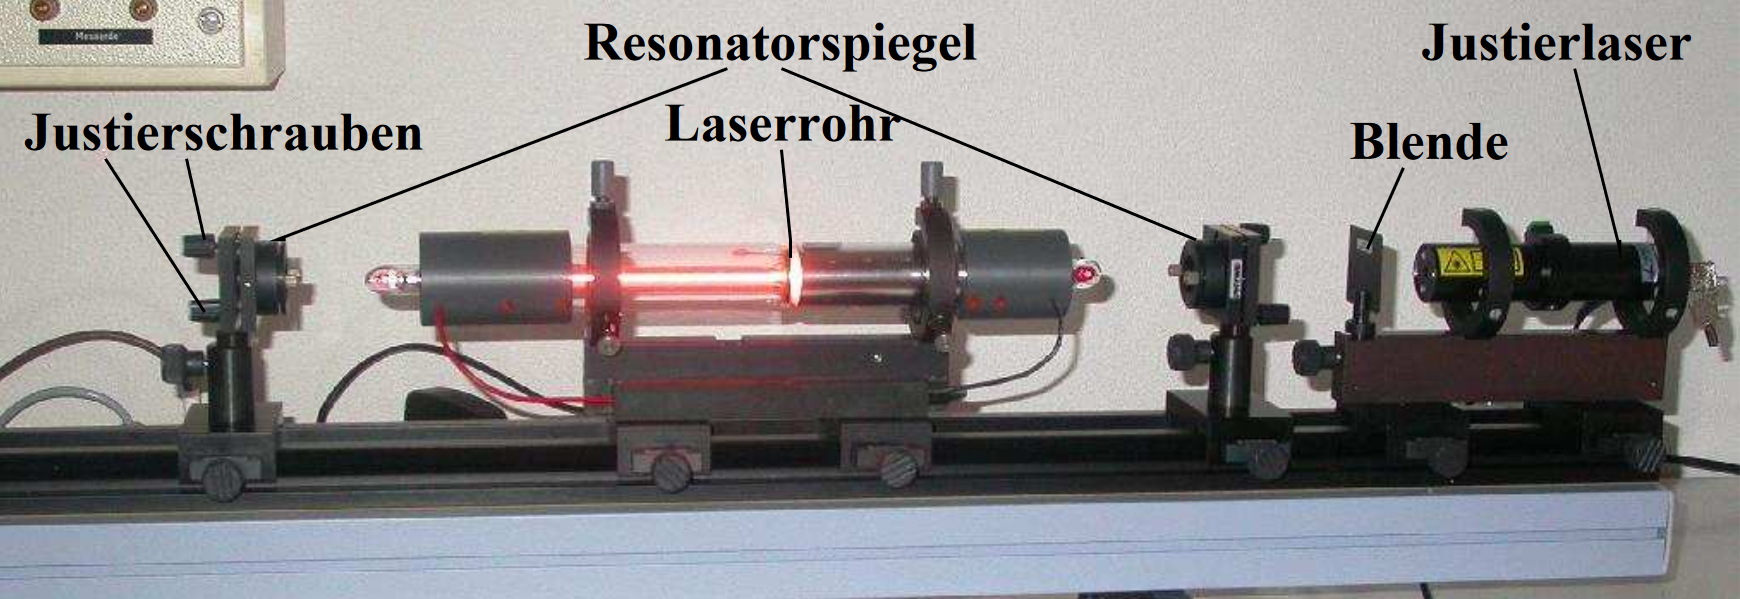
\includegraphics[width=\linewidth-100pt,height=\textheight-100pt,keepaspectratio]{content/Images/aufbau.png}
	\caption{Experimenteller Aufbau \cite{V61}.}
	\label{fig:Aufbau}
\end{figure}

Der Laser wird auf einer optischen Schiene aufgebaut. Auf dieser befindet sich ein Justierlaser der zur Justierung der anderen Komponenten benötigt wird. Weiterhin ist ein Laserrohr, welches mit dem HeNe-Gasgemisch gefüllt ist, auf der Schiene befestigt. Das Laserrohr ist auf beiden Seiten mit Brewsterfenstern abgeschlossen. Die Elektroden des Laserrohrs, die für die Gasentladung sorgen, sind an eine Spannungsquelle angeschlossen. Auf beiden Seiten neben dem Laserrohr sind die hochreflektiven Spiegel des Resonators angebracht. Weiterhin können zur Untersuchung des Lasers weiter eine Photodiode, ein Gitter und ein Polarisationsfilter in den Laserstrahl eingebracht werden. Zur Stabilisierung der  $\text{TEM}_{mnq}$-Moden kann ein Draht in den Resonator eingebracht werden.